% Deben explicarse los metodos numericos que utilizaron y su aplicacion al
% problema concreto involucrado en el trabajo practico. Se deben mencionar los
% pasos que si- guieron para implementar los algoritmos, las dicultades que
% fueron encontrando y la descripcion de como las fueron resolviendo. Explicar
% tambien como fueron planteadas y realizadas las mediciones experimentales.
% Los ensayos fallidos, hipotesis y conjeturas equivocadas, experimentos y
% metodos malogrados deben gurar en esta seccion, con una breve explicacion
% de los motivos de estas fallas (en caso de ser conocidas)

\section{Implementación}

Para realizar el análisis de los métodos y funciones previamente descriptos
realizamos una implementación en \verb|C| que nos permite decidir
paramétricamente cómo resolver la inversa de la raíz de un número dado.\\

La implementación acepta los siguientes parámetros:

\begin{itemize}
    \item Función $e(x)$ o $f(x)$
    \item Método de Newton o de la Secante
    \item Criterio de parada:
    \begin{itemize}
        \item Cantidad de iteraciones
        \item Tiempo de Ejecución
        \item Error Absoluto
        \item Error Relativo
    \end{itemize}
    \item Eleccion de $x_0$ y $x_1$ ($x_1$ solo para el método de la Secante)
\end{itemize}

Luego de obtenido el resultado en base a los parámetros elegidos nuestra
implementación devuelve:

\begin{itemize}
    \item la aproximación en cada iteración
    \item el error absoluto
    \item el error relativo
    \item el tiempo de ejecución
\end{itemize}

Realizamos también unos helpers en \verb|Python| para poder crear experimentos
de forma sencilla, poder replicarlos cuantas veces sea necesario y analizar
los resultados.\\

El código escrito se puede optimizar \textbf{mucho}, sobre todo en las cuentas
que realiza el cuerpo de cada metodo. Ahora hay una implementación naive que
replica el enfoque analítico pero que a nivel cantidad y complejidad de
operaciones se puede mejorar.\\

Por otro lado, hay un alto grado de overhead debido a la forma que decidimos
implementar la flexibilidad de ejecución con los parámetros elegidos, pero
podemos ver que esto afecta a los dos métodos y funciones por igual por lo que
no debería afectar las comparaciones y resultados.

\newpage
\section{Desarrollo}

Decidimos analizar las siguientes combinaciones entre métodos y funciones para
calcular la inversa de la raíz de un número:

\begin{itemize}
    \item raíz de $f(x)$ aproximada mediante el método de Newton
    \item raíz de $e(x)$ aproximada mediante el método de Newton
    \item raíz de $e(x)$ aproximada mediante el método de la Secante
\end{itemize}

Recordemos que para el caso de estas funciones, es lo mismo encontrar
cualquiera de sus raices ya que tienen igual módulo y encontrando raíz se puede
encontrar la otra cambiando el signo (\ref{sec:analisis_f_x}
y~\ref{sec:analisis_e_x}).

\subsection{Ajuste de parámetros}

Cada una de estas variantes tiene parámetros según el método utilizado que se
pueden ajustar según la función a analizar. En particular para el método de
Newton hay que elegir una primera aproximación $x_0$ en base a $f(x)$ o $e(x)$
(que puede o no ser la misma) y para el método de la Secante y $e(x)$ hay que
elegir $x_0$ y $x_1$.

Decidimos realizar nuestro análisis enfocados en una amplia gama de magnitudes
de números a los cuales les queremos buscar la inversa de la raíz. Estamos
interesados tanto en números muy pequeños, cercanos al cero y en números muy
grandes, lejanos del 0.

Por esta razón, para el ajuste de parámetros decidimos utilizar un criterio de
parada de error relativo entre iteraciones. Gracias a esta elección y el
caracter iterativo de los métodos a utilizar nos garantizamos que no importa la
magnitud del número dado, siempre encontraremos una solución con un error
relativo al resultado pequeño, por lo que los parámetros a elegir nos deben
otorgar buenos resultados para números muy grandes y muy pequeños.

\subsubsection{Ajuste de $x_0$ para $f(x)$ y el método de Newton}

Al buscar una raíz de $f(x)$ mediante el método de Newton tenemos asegurada la
convergencia para cualquier $x_0$ mayor a alguna de las raices
(\ref{sec:convergencia}). Al saber que existen dos raíces de igual módulo
podemos elegir $x_0 = 0 + \epsilon$ y tener garantizada la convergencia. Notar
que no se puede elegir $x_0 = 0$ ya que la recta tangente en ese punto es
constante y no se interseca con el eje de las abscisas. No obstante un análsis
analítico nos puede permitir elegir un mejor $x_0$.

\begin{figure}[!htbp]
  \begin{center}
    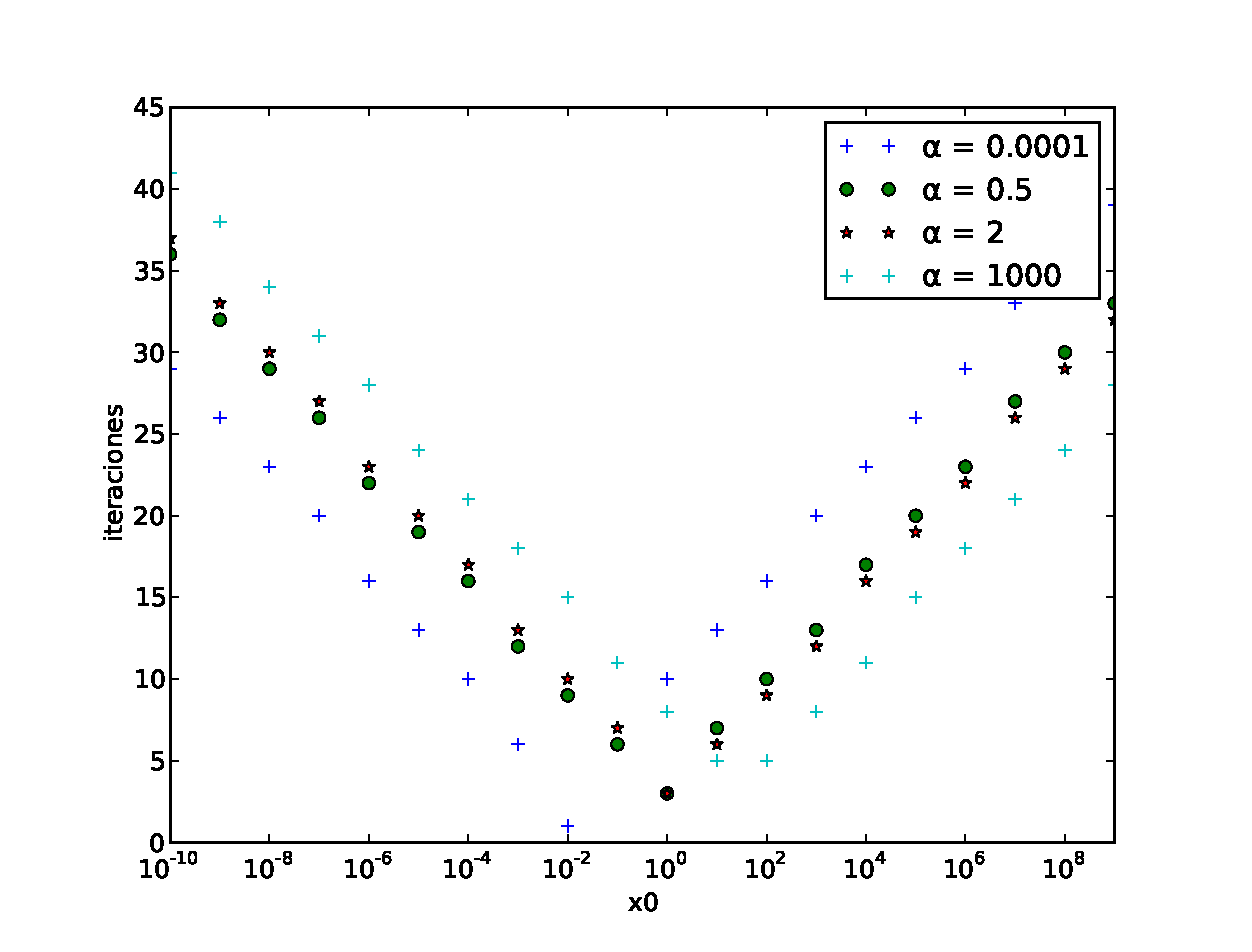
\includegraphics[scale=0.5]{graficos/new/f_newton_x0_variable.eps}
    \caption{\label{fig:f_newton_x0_variable} Gráfico de cantidad de iteraciones fijando $\alpha$ variando $x_0$ para $f(x)$ utilizando el método de Newton.}
  \end{center}
\end{figure}

En la Figura~\ref{fig:f_newton_x0_variable}  podemos ver como varía la cantidad
de iteraciones, cambiando la magnitud de $x_0$. Cuando $x_0$ es muy grande
empezamos muy lejos de la solución, con lo cual se requieren muchas iteraciones
para llegar al resultado.\\

Cuando $x_0$ es muy pequeño, cercano al $0$, la pendiente de la tangente a
$f(x)$ es cercana al 0, por lo que en la siguiente iteración $x_1$, el punto donde
esta recta se interseca con el eje de las abscisas es muy grande, cayendo en el
caso anterior partiendo desde $x_1$ de un punto muy grande, con un valor muy
alejado de la solución.

\begin{figure}[!htbp]
  \begin{center}
    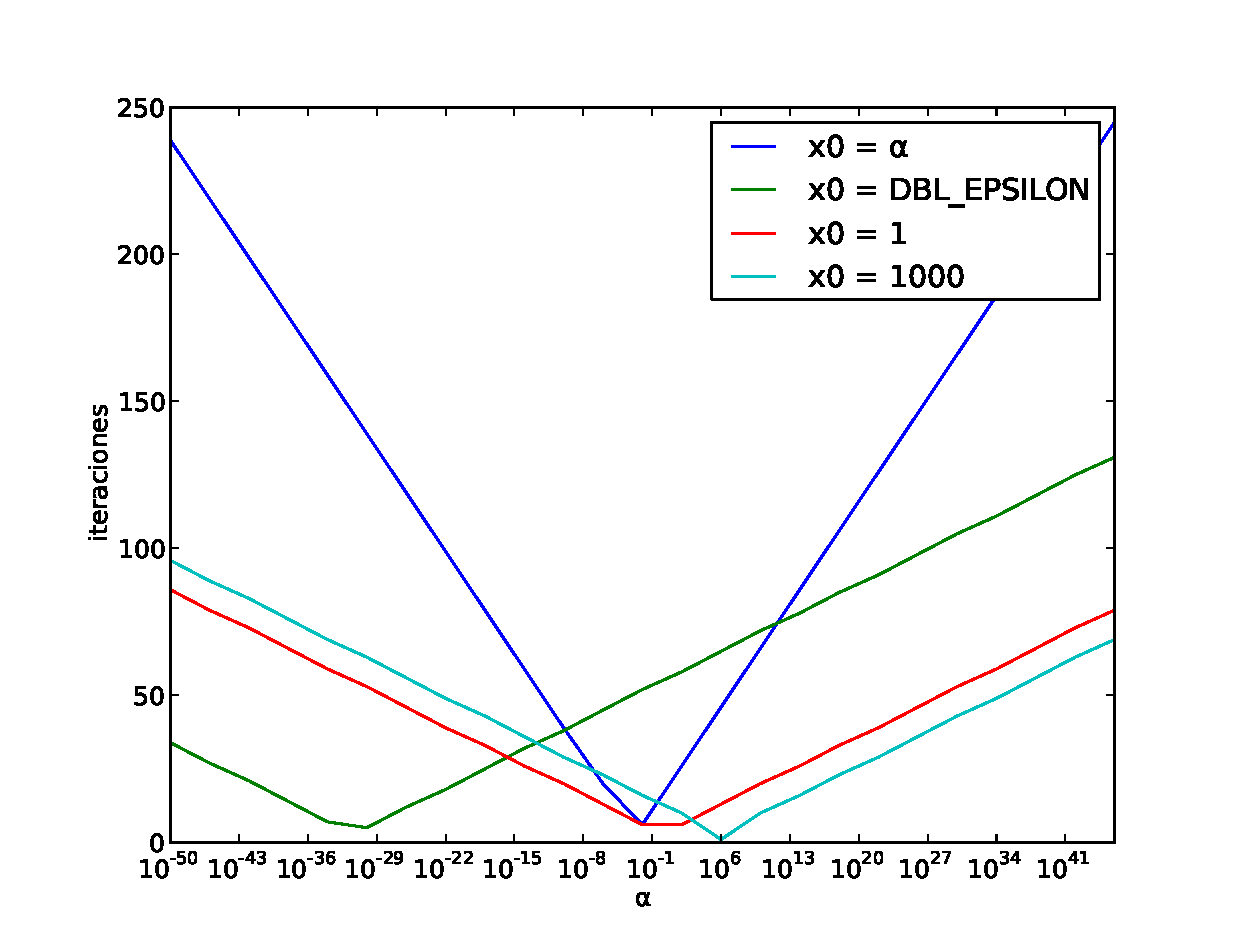
\includegraphics[scale=0.5]{graficos/new/f_newton_x0_fijo_1.eps}
    \caption{\label{fig:f_newton_x0_fijo_1} Gráfico de cantidad de iteraciones fijando $x_0$ variando $\alpha$ para $f(x)$ utilizando el método de Newton.}
  \end{center}
\end{figure}

En la Figura~\ref{fig:f_newton_x0_fijo_1} graficamos la cantidad de iteraciones
necesarias para llegar al resultado, fijando diferentes puntos de partida $x_0$
y variando la magnitud de $\alpha$. Las variantes que mostramos en esta figura
son $x_0$ constantes y en función del $\alpha$. Una de las opciones de $x_0$ es
$\textit{DBL\_EPSILON}$; dependiente de nuestra implementación particular es el
menor número tal que $1.0 + \textit{DBL\_EPSILON} \ne 1.0$. En nuestro caso, es
el menor $x_0$ positivo que podemos utilizar sin entrar en errores de pérdida
de dígitos significativos. Luego incluímos las opciones constantes de $x_0 = 1$
y $x_0 = 1000$. Por último incluímos un $x_0$ linealmente dependiente de $\alpha$.\\

Se puede observar claramente que $x_0$ con valores constantes crecen más
lentamente que $x_0 = \alpha$ para la gran mayoría de valores. Intentamos
probar también con $x_0 = 1 / \alpha$ pero para valores muy chicos encontramos
rápidamente errores de pérdida de dígitos significativos y para valores grandes
no se observaban beneficios.

\begin{figure}[!htbp]
  \begin{center}
    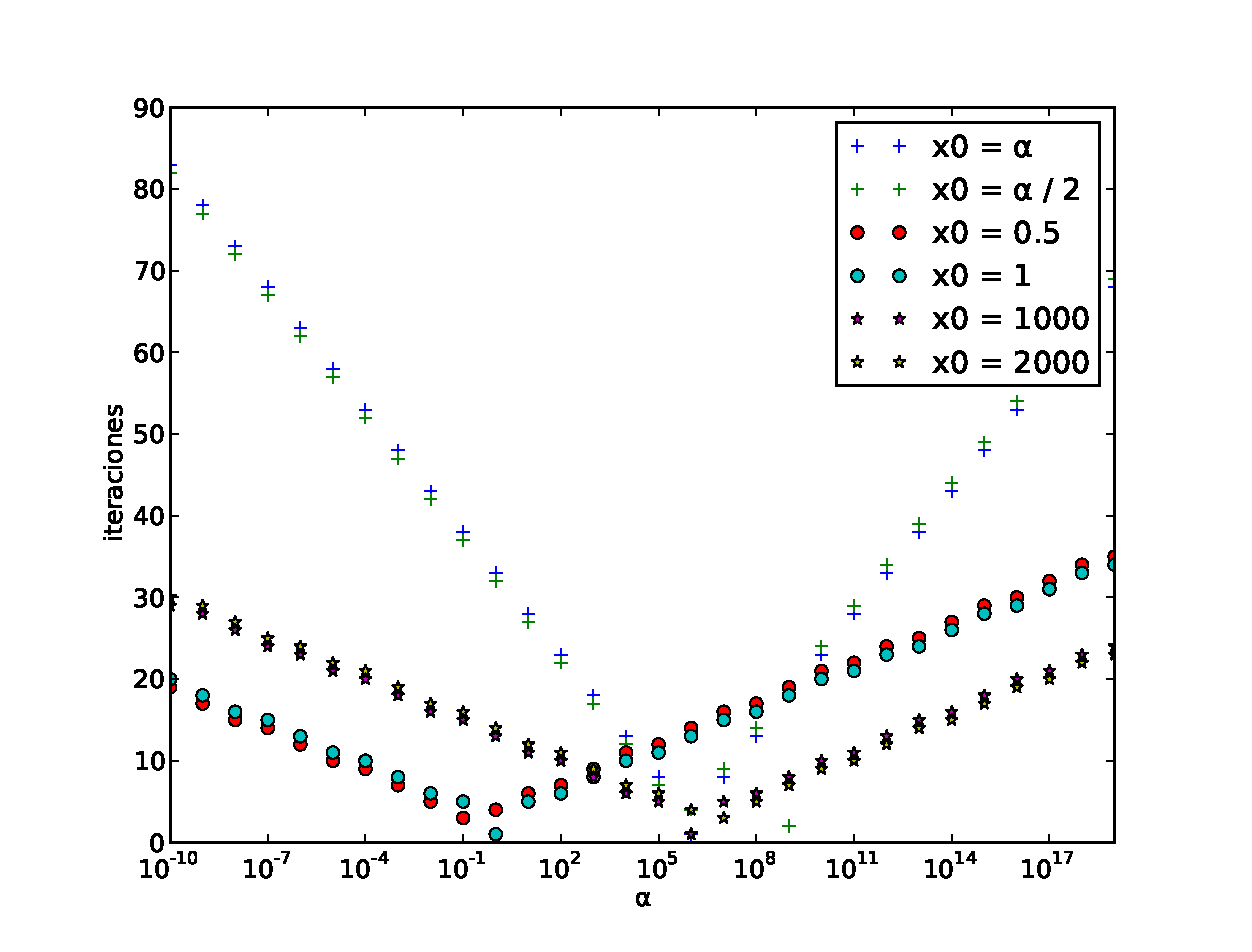
\includegraphics[scale=0.5]{graficos/new/f_newton_x0_fijo_2.eps}
    \caption{\label{fig:f_newton_x0_fijo_2} Gráfico de cantidad de iteraciones fijando $x_0$ variando $\alpha$ para $f(x)$ utilizando el método de Newton (más variantes).}
  \end{center}
\end{figure}

En la Figura~\ref{fig:f_newton_x0_fijo_2} graficamos algunos valores más para
$x_0$ variando las constantes utilizadas. Se observa claramente que variar la
constante produce un \emph{corrimiento} de la cantidad de iteraciones lo cual
tiene sentido ya que se empieza cerca del resultado para diferentes valores de
$\alpha$. Este corrimiento se realiza en base a la magnitud (o valore relativo)
de $x_0$ y no en base a su valor, lo que implica que el corrimiento entre $x_0
= 0.5$ y $x_0 = 1$ es similar al corrimiento entre $x_0 = 1000$ y $x_0 = 2000$
ya que diferencia relativa entre estos valores es de $1/2$.\\

Se puede observar también que tomando diferentes $x_0$ en relación lineal con
$\alpha$ también produce un corrimiento y no una diferencia en la pendiente.\\

En base a estos resultados decidimos tomar $x_0 = 1$ para calcular $f(x)$
utilizando el método de Newton ya que mantiene un equilibrio entre magnitudes
muy grandes y magnitudes muy pequeñas.

\subsubsection{Ajuste de $x_0$ para $e(x)$ y el método de Newton}

A diferencia de $f(x)$ para el método de Newton, no contamos con seguridad en
la convergencia de este método para esta función. En las figuras que mostramos
a continuación sólo graficamos los valores para los cuales el método converge,
por esto se verán sectores de cada variante no graficados.

\begin{figure}[!htbp]
  \begin{center}
    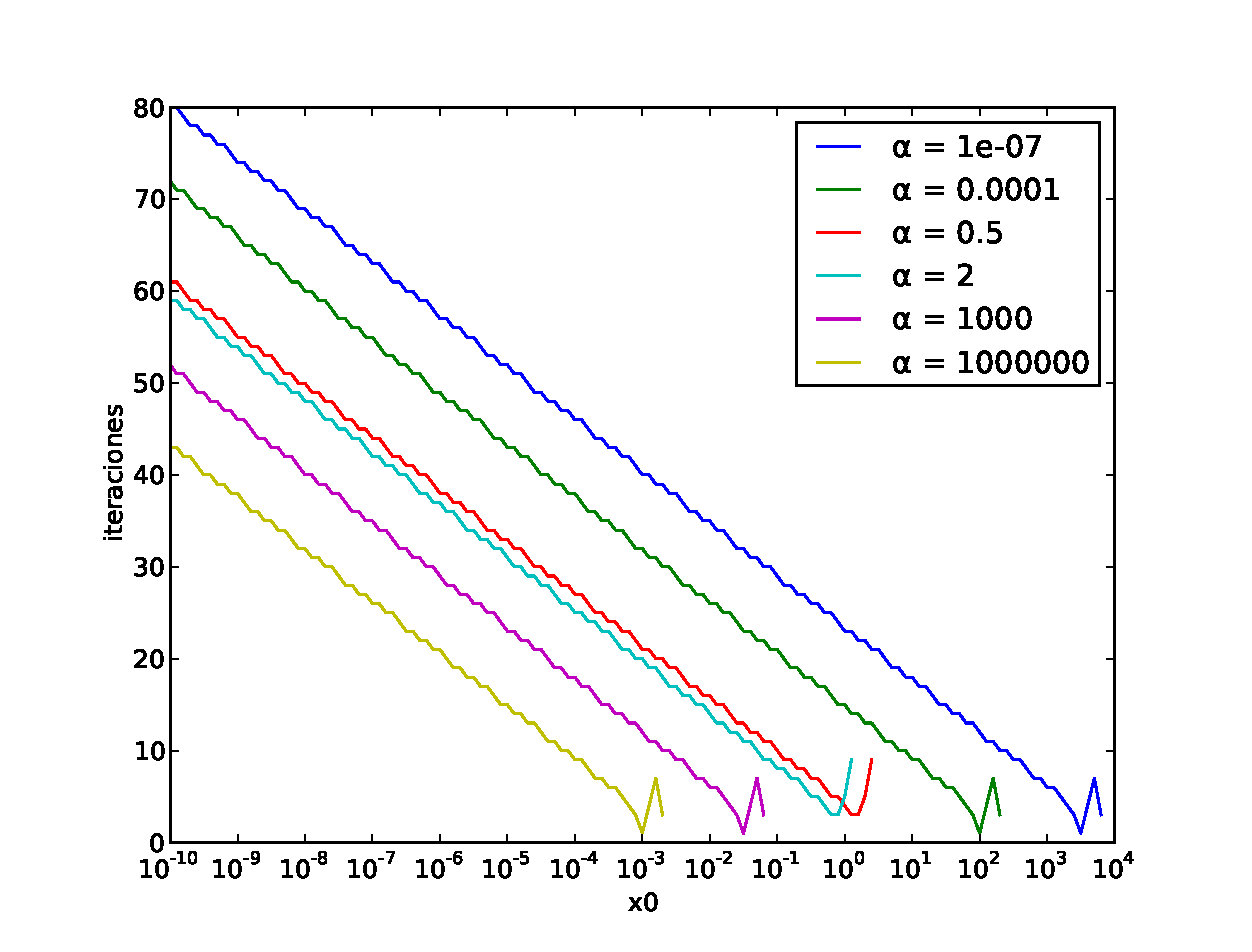
\includegraphics[scale=0.5]{graficos/new/e_newton_x0_variable.eps}
    \caption{\label{fig:e_newton_x0_variable} Gráfico de cantidad de iteraciones fijando $\alpha$ variando $x_0$ para $e(x)$ utilizando el método de Newton.}
  \end{center}
\end{figure}

En la Figura~\ref{fig:e_newton_x0_variable} lo primero que podemos observar es
como pensado que no todos los $\alpha$ convergen para todos los $x_0$. Cuanto
mayor es el $\alpha$ necesitamos un mayor $x_0$ para lograr la convergencia. No
obstante, si fijamos un $x_0$ constante muy grande, la cantidad de iteraciones
necesarias para llegar al resultado para $\alpha$ chicos es muy grande.\\

Se nos ocurren dos alternativas posibles del porqué no converge hacia el
resultado. La primera es que simplemente el método no converge para todos los
$x_0$ para todos los $\alpha$ ya que no tenemos un análisis que lo garantice.
La segunda alternativa es que al poseer dos asíntotas, al variar poco algunos
números varía mucho hacia números \textbf{muy} grandes la intersección con las
abscisas de las tangentes o la evaluación de $e(x)$ en valores cercanos al $0$.
Esto puede producir la pérdida de dígitos significativos perjudicando la
convergencia. Para muchas de las pruebas que realizamos durante la
implementación obtuvimos valores intermedios donde la representación de doble
punto flotante nativa utilizada llegaba a $\infty$.

\begin{figure}[!htbp]
  \begin{center}
    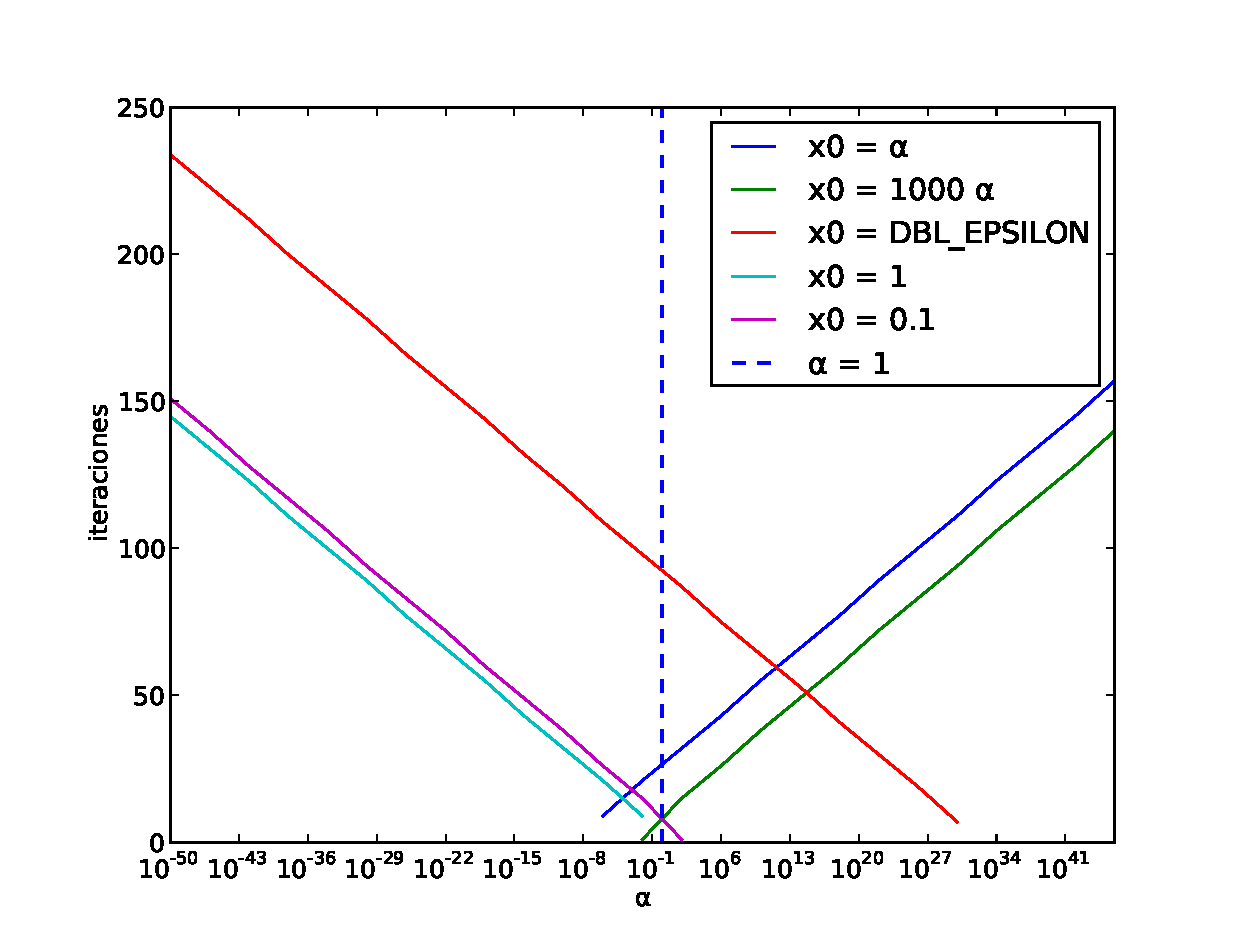
\includegraphics[scale=0.5]{graficos/new/e_newton_x0_fijo.eps}
    \caption{\label{fig:e_newton_x0_fijo} Gráfico de cantidad de iteraciones fijando $x_0$ variando $\alpha$ para $e(x)$ utilizando el método de Newton.}
  \end{center}
\end{figure}

En la Figura~\ref{fig:e_newton_x0_fijo} podemos observar cómo se comporta la
cantidad de iteraciones y la convergencia de diferentes $x_0$ mientras variamos
la magnitud de $\alpha$. Decidimos probar al igual que en el análisis del
método de Newton para $f(x)$ el comportamiento con $x_0 =
\textit{DBL\_EPSILON}$. En este caso, converge para gran cantidad del dominio
pero necesita muchas iteraciones para $\alpha$ pequeños. En el caso de $x_0 =
\alpha$ podemos observar que converge para valores muy grandes de $\alpha$.\\

Notemos que parecen generar pendientes similares pero invertidas.\\

Utilizar otras constantes para $x_0$ o multiplicar $\alpha$ por una constante
genera nuevamente un ``corrimiento'' sin cambio perceptible en la pendiente.\\

En un análisis de la forma de la función pensamos en utilizar $x_0 = 1 /
\alpha$ pero en la práctica no converge.\\

Al igual que en el caso anterior decidimos tomar valores para ``equilibrar''
diferentes magnitudes de $\alpha$ alrededor del $1$. Para esto buscamos
mediante una búsqueda binaria (manual) los valores para $x_0$ para producir la
menor cantidad de iteraciones en $\alpha = 1$. Los valores encontrados y que
utilizaremos para $e(x)$ y el método de Newton son:

\[
\begin{cases}
x_0 = 0.1, & \mbox{si } \alpha < 1\\
x_0 = \alpha * 1000, & \mbox{si } \alpha \ge 1
\end{cases}
\]

La cantidad de iteraciones para estos valores se pueden observar en la
Figura~\ref{fig:e_newton_x0_fijo} donde se encuentra graficada su intersección
en $\alpha = 1$.

\subsubsection{Ajuste de $x_0$ y $x_1$ para $e(x)$ y el método de la Secante}

En el caso del método de la secante para $e(x)$ debemos elegir tanto $x_0$ como
$x_1$. En esta combinación tampoco tenemos asegurada la convergencia. Al igual
que en el apartado anterior, en las figuras que mostramos a continuación sólo
graficamos los valores para los cuales el método converge.\\

El enfoque que decidimos tomar para esta combinación es el siguiente: Teniendo
en cuenta que el método de la Secante se puede ver como una aproximación por
diferencias finitas del método de Newton, intentamos replicar los resultados,
eligiendo los mismos $x_0$ y ajustando los $x_1$ para obtener valores
similares.

\begin{figure}[!htbp]
  \begin{center}
    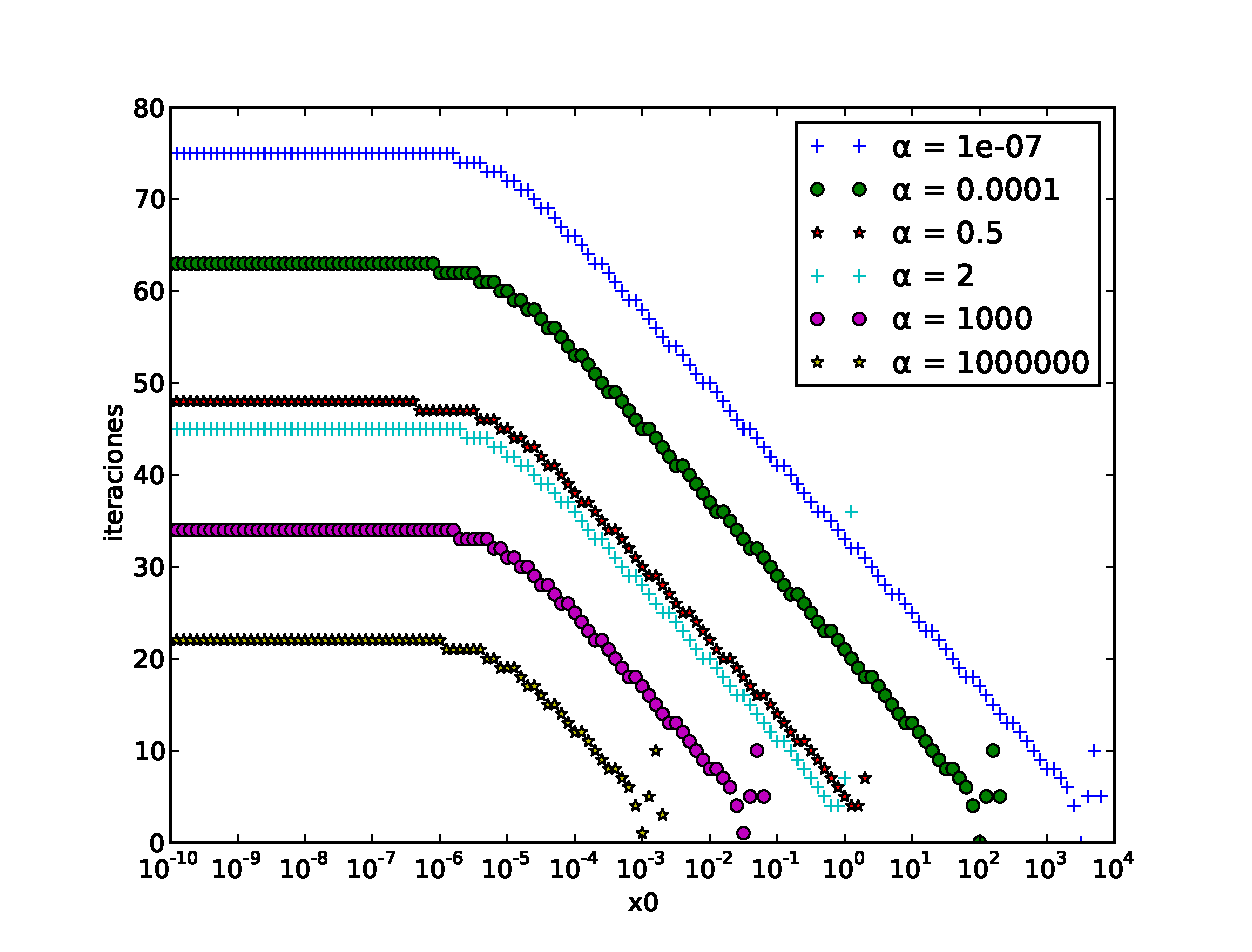
\includegraphics[scale=0.5]{graficos/new/e_secante_x0_variable.eps}
    \caption{\label{fig:e_secante_x0_variable} Gráfico de cantidad de iteraciones fijando $\alpha$ variando $x_0$ para $e(x)$ utilizando el método de la Secante.}
  \end{center}
\end{figure}

En la Figura~\ref{fig:e_secante_x0_variable} podemos observar resultados
similares a los de la Figura~\ref{fig:e_newton_x0_variable}. Al igual que en
esta no todos los $\alpha$ convergen para todos los $x_0$. Las mismas
conclusiones aplican, cuanto mayor es el $\alpha$ necesitamos un mayor $x_0$
para lograr la convergencia a costa de mayor cantidad de iteraciones para
$\alpha$ chicos.\\

Los $x_1$ tomados para este experimiento son $x_1 = x_0 + 0.0001$. Al elegir
estos $x_1$ cercanos a los $x_0$ la idea fue aproximar la tangente obtenida en
la primera iteración del método de Newton. Puntos $x_1$ más cercanos a $x_0$
producían una menor convergencia en el mismo dominio.\\

Se puede observar también como la cantidad de iteraciones crece a medida que el
$\alpha$ crece hasta un punto donde la cantidad de iteraciones se mantiene
estable. Creemos que esto se debe a las asíntotas, donde la elección de $x_0$ y
$x_1$ tan grandes producen muy poca variación en el cálculo de la tangente.\\

Se puede notar también una mayor cantidad de iteraciones necesarias para
alcanzar los mismos resultados que para el método de Newton, lo que concuerda
con la el grado de convergencia teórico.

\begin{figure}[!htbp]
  \begin{center}
    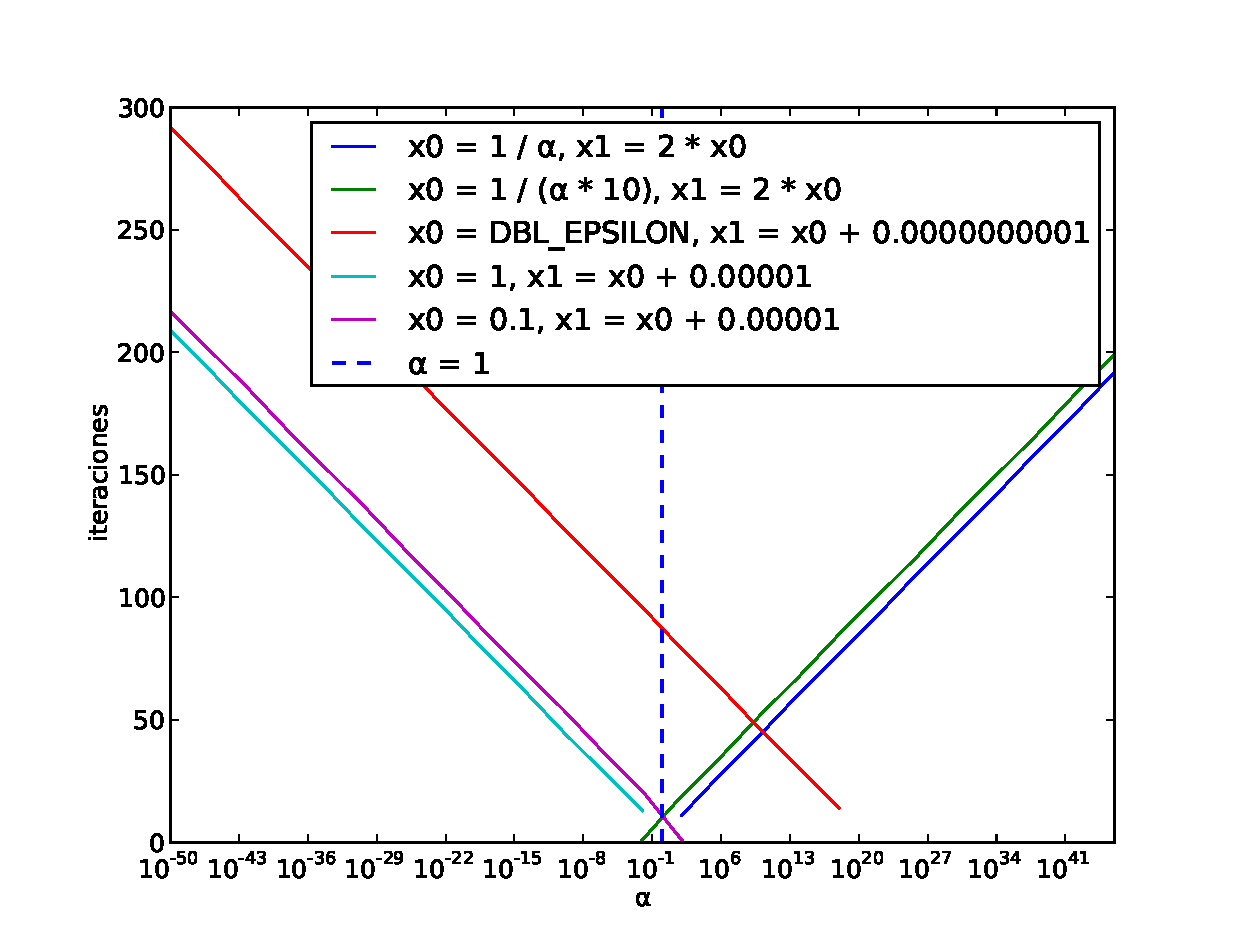
\includegraphics[scale=0.5]{graficos/new/e_secante_x0_fijo.eps}
    \caption{\label{fig:e_secante_x0_fijo} Gráfico de cantidad de iteraciones fijando $x_0$ variando $\alpha$ para $e(x)$ utilizando el método de la Secante.}
  \end{center}
\end{figure}

En la Figura~\ref{fig:e_secante_x0_fijo} podemos observar cómo se comporta la
cantidad de iteraciones y la convergencia de diferentes $x_0$ mientras variamos
la magnitud de $\alpha$. Decidimos probar al igual que en la
Figura~\ref{fig:e_newton_x0_fijo} el comportamiento con $x_0 =
\textit{DBL\_EPSILON}$. Para lograr el mismo dominio de convergencia
necesitamos utilizar un $x_1$ aún más cercano,  $x1 = \textit{DBL\_EPSILON} +
0.0000000001 = x_0 + 0.0000000001$.\\

Para los casos donde $x_0$ es un múltiplo de $\alpha$ fue necesario multiplicar
$x_1 = 2 \times x_0$ para lograr el mismo dominio de convergencia que en el método
de Newton.\\

Estos resultados mantienen la misma forma que los de la
Figura~\ref{fig:e_newton_x0_fijo}, incluso los valores de $x_0$ se mantienen
para lograr ``equilibrar'' la convergencia en $\alpha = 1$.\\

Los valores encontrados y que utilizaremos para $e(x)$ y el método de la
Secante son:

\[
\begin{cases}
x_0 = 0.1 \wedge x_1 = x_0 + 0.00001, & \mbox{si } \alpha < 1\\
x_0 = \alpha * 1000 \wedge x_1 = x_0 * 2, & \mbox{si } \alpha \ge 1
\end{cases}
\]

La cantidad de iteraciones para estos valores se pueden observar en la
Figura~\ref{fig:e_secante_x0_fijo} donde se encuentra graficada su intersección
en $\alpha = 1$.

\subsection{Análisis práctico de convergencia}

En esta sección estudiaremos de forma práctica la convergencia de cada uno de
los métodos y la compararemos con la convergencia teórica.
